%
% Latex Document made by TheInevitables for SRS,  COS 301 2017
%

\documentclass{article}


\usepackage{geometry}
\usepackage[utf8]{inputenc}
\usepackage{graphicx}
\usepackage{float}
\usepackage{amsmath}
\usepackage{amsfonts}
\usepackage{amssymb}
\usepackage{graphicx}
\usepackage{float}
\usepackage[explicit]{titlesec}
\usepackage{url}


\DeclareGraphicsExtensions{.png}
\DeclareGraphicsExtensions{.jpg}
\graphicspath{ {Diagrams/} }

 \geometry{
 a4paper, 
 total={170mm, 257mm}, 
 left=25mm, 
right=25mm, 
 top=25mm, 
 }
 
 \title{ Software Requirements Specification \\ COS-301 \\ The Inevitables \\[0.5cm] 
\includegraphics[width=6cm]{front-page}}
 
 \author{Drew Langley \hfill 11039753 \\ Lyle Nel \hfill 29562695 \\ Dawie Pritchard \hfill 13104340 \\  Peter Rayner \hfill 14001757\\ Hendrik Jan van der Merwe \hfill 15101283 \\ [1cm]\includegraphics[width=10cm]{Diagrams/group.JPG}\\ [1cm] Clients: Morkel Theunissen and Maria Ramaahlo }
\date{23 May 2017}


\begin{document}
\maketitle
\pagebreak
\tableofcontents
\pagebreak

%%%%%%%%%%%%%%%%%%%%%%% =========== INTRODUCTION ================== %%%%%%%%%%%%%%%%%%%%%%%%%%%%

\section{Introduction}
		Many mobile applications exist to assist their users in successful travel from one location to another, by vehicle, or on foot. \\
		Though these applications exist and work very well, solutions for disabled persons such as visual and physical impairments do not exist.\\ \par
		This document serves to formally introduce and quantify the Object Sensor and Mobile Navigation application, this project is part of the COS 301 (Software Engineering) Capstone project available for bid in 2017. This project was successfully tendered by TheInevitables.
	
	\subsection{Purpose}
		The purpose of this document is to provide a detailed description of the requirements presented by the Object Sensor and Mobile Navigation application, this application is intended to assist the students of the disability unit with navigation around the University of Pretoria. Additionally this document will include possible constraints and technical requirements such as how the system wil interact with external applications, such as the users. \par
		This document is intended to comply with the IEEE 830-1998 SRS Standard. This document is also intended for use by clients Morkel Theunissen and Maria Ramaahlo for approval such that the system implementation may begin.
		
	\subsection{Scope}
%		The orientation and navigation of students with visual disabilities is essential to them accessing the academic environment. Whilst, many students with visual disabilities may make use of trained guide dogs or canes, additional support is required when navigating their way through the many obstacles on campus. This includes but is not limited to poles, low hanging roofs,bollards and other objects.\\
%		The Object Sensor and Mobile Navigation application will make use of GPS, GIS and WiFi access point data to determine the current location of a user and safely navigate them to their destination on the University of Pretoria's campus facilities, this includes but is not limited to lecture halls, laboratories, food courts, ablutions and so on. The system will also make use of fiducial markers which will be used to notify the user of an impending obstacle.

		
	\subsection{Definitions, Acronyms and Abbreviations}
		\begin{itemize}
			\item IEEE - Institute of Electronic and Electrical Engineers.
			\item GPS - Global Positioning System.
			\item GIS - Geographic Information System.
			\item WiFi - Wireless Fidelity.
			\item WCAG - Web Accessibility Guidelines.
			\item AR Tag - An Augmented Reality Tag that is printable and facilitates physical tagging to be read using machine vision at a later stage.
			\item ArUco - A specific binary square fiducial marker implementation that that is the main candidate for AR Tagging in this project.
			\item Fiducial marker - A machine readable object in the physical world that is used to tag objects that are deemed relevant the navigation system.
		\end{itemize}
		
		The DU@UP Object Sensor and Mobile Navigation application will be from hereforth reffered to as NavUP.
		
	\subsection{References}
		\begin{itemize}
			\item IEEE 830-1998 SRS Standard - \url{https://standards.ieee.org/findstds/standard/830-1998.html}
			\item DU@UP Object Sensor and Mobile Navigation - \url{}
		\end{itemize}
	
\newpage
%	\subsection{Project background}
%		The orientation and navigation of students with visual disabilities is essential to them accessing the academic environment. Whilst, many students with visual disabilities may make use of trained guide dogs or  canes, additional support is required when navigating their way through the many obstacles on campus. This includes but is not limited to poles, low hanging roofs ,bollards and other objects.
%
%	\subsection{Project vision}
%The development of mobile communications allows for the development of applications for the independent navigation of persons with visual disabilities. The combination of mobile technologies, navigation systems and low tech devices will assist students to safely and successfully navigate their way on campus.	
%	
	\subsection{Overview}
		These are the sections that follow; \\
		The Overall Description, which describes the overall system, the modules and the interfaces that exist within the system, the system functions, the characteristics of the users, the systems' possible constraints and the assumptions and dependencies required for the system.\par
		The Functional Requirements section lists the requirements the system should adhere to and describes use cases.\par
		The Specific Requirements section is mainly intended for developers and is dedicated to defining the external interface requirements, functional requirements, performance requirements, design constraints, quality requirements and software system attributes. \par
		The development of mobile communications allows for the development of applications for the independent navigation of persons with visual disabilities. The combination of mobile technologies, navigation systems and low tech devices will assist students to safely and successfully navigate their way on campus.	
		 

%%%%%%%%%%%%%%%%%%%%%%============== OVERALL DESCRIPTION ==============%%%%%%%%%%%%%%%%%%%%%%%%%%%%
\newpage
\section{Overall Description}

	\subsection{Product Perspective}
		Similar to existing navigation applications such as Google Maps and Waze, the NavUP is a standalone mobile application that acts as a campus navigation system for students both with and without disabilities. It encompasses many technologies which will be required to provide the requested and necessary functionality as described in the functional requirements section.\\ \par
		Obstacles described previously such as poles and low hanging roofs, intersections on campus(between IT Bulding and EB building) will be fitted with fiducial markers. These markers will be detected using machine vision and will be used to warn users when they are in proximity to certain obstacles or landmarks.\par
		The system will use the user's smart device's hardware interfaces such as GPS to accurately get the user's location data, and navigate them to their required destination.\\
		
	\subsection{Product Functions}
		The NavUp system will support a variety of functions, the main function focuses on reliable, accurate navigation and presentation of geographical data, both indoors and outdoors. Other functionality includes providing information, and special routes for students with disabilities.
		\\ \par
		The navigational functionality will consist of getting the user's current destination accurately and then determining a suitable route to the venue the user requests.\\ \par
		Students with visual disabilities already have defined routes which the system must cater for.\\ \par
		Information provided to users will consist of venue information, geographical information, and information regarding the proximity of obstacles to visually impaired users.\\ \par
		Users will be given the fastest route to their destination, unless they are physically impaired, which results in a route that takes lifts and wheelchair access into account.\\ \par
		Due to the project focusing on the assistance of visually and physically impaired students and users, the application will conform to the WCAG to ensure these users with ease of use and accessibility.\\ \par
		The system will be developed to run on mobile devices, and will be acquired by users from the "Google Play Store".\\ \par
		The application will be percievable, operable, reliable and follow the University of Pretoria's colour scheme and branding guidelines visually.\\ \par
		Normal users will have the option to notify the system of a potential hazard or obstacle to impaired students. This will be accomplished by allowing them to drop a location pin and wil work as a crowdsourcing technique to identify and capture dynamic obstacles. \\ \par
		The application will also be secure to avoid theft or loss of data.
			
	\newpage
	\subsection{User Characteristics}
		The main category of individuals that will make use of NavUP will be designed for will be visually impaired students of the University of Pretoria.\\
		The main body of students and staff will also have access to the application.
		These students will interact with the system via the mobile application. This means they will not require information regarding how the software works, however it is important to keep their information safe. They will also be required to have access to and knowledge of how to use a smart device.\\ \\
		Other users would include maintenance workers and administrative users, responsible for updating information pertaining to the application. These administrators will require knowledge about how the software works so as to maintain it correctly.
	
	
	
	\subsection{Constraints}
		The following is a list of possible design constraints related to NavUP:
		
			\begin{itemize}
				\item Security  - The users personal information and current location should not be accessible to the public.
				\item Accuracy - The users location should be found whether the user is indoors or not. The location of the user should also be found in terms of which floor they are on in the building.
				\item Performance - The system should be able to handle a large amount of users making use of the software at the same time.
				\item Reliability - The application should still operate when one or more data access points are no longer available.
				\item Accessibility - The application should be easily accessible to everyone that requires it.
				\item Usability - The applications interface should be easy to use and understand.
				\item Size - The application should not require too much memory in order to operate.
				\item Users - The nature of some users enforces constraints such as conforming to the WCAG for accessibility issues.
			\end{itemize}
	
	
	\subsection{Assumptions and Dependencies}
		The application will be developed to operate from a user's smart device, these smart devices usually have all the necessary hardware fitted. It is therefore assumed that all users of the NavUP will have access to one of these smart devices. It is then assumed that these devices have the required hardware dependencies and capabilities to run the application correctly. Such dependencies and hardware include WiFi, GPS and cellular network data connectivity.\\ \\
		It is also assumed that the users will be students of the university, thereby having access to the information regarding their venues and times is provided to them.\\
		In terms of usability, it is assumed the users will have knowledge regarding how to use mobile devices and their applications, this includes activating voice controls and so on. \\ \\
		Assumptions relating to the system itself include the beliefs that the system will be kept up to date with the latest venue information and GIS data. It is also assumed that the fiducial markers will always be operational. These dependencies relate to the accuracy and relaibility of the system and it is therefore assumed and recommended that a maintenance schedule be put in place.\\
		A final assumption relating to continuous, relaible performance of the application is dependent on server capacity.
		
		
		

\newpage
%%%%%%%%%%%%%%%%%%%%%%%============= Functional Requirements =================%%%%%%%%%%%%%%%%%%%%%%%%%
\section{Functional Requirements}
%\begin{itemize}
%	\item Navigation through the use of WiFi Access point data
%	\item Functionality across Android devices
%	\item The application should be developed to function on Google's Play Store.
%	\item Compliance with most recent web accessibility guidelines
%	\item The application should be perceivable, operable, understandable and robust
%	\item Machine vision will be used to detect fiducial markers
%	\item Has to make use of voice recognition technology
%	\item fiducial markers should determine localization and distance from user device
%	\item fiducial markers should notify users of impending obstacles such as bollards
%\end{itemize}

		\subsubsection {REQ1: Navigation}
			Provide navigation functionality.\\ This involves getting a users current position accurately and providing a route to the user's destination.
			
		\subsubsection{REQ2: Usability}
			The system should allow all kinds of users access to helpful navigational information. These users include students, visually and physically impaired students, staff and guests. This involves accessibility and usability issues.
			
		\subsubsection{REQ3: Provide Different Routes}
			Provide different routes based on the user's needs and preferences. This could be for physically or visually impaired users, or by a request for the fastest route taking stairs, ramps, lifts, wheelchair access and obstacles into consideration. %This wil require the use of fiducial markers and data capture such as locations of wheelchair ramps/lifts and the machine vision section to detect obstacles.
			
		\subsubsection{REQ4: Mobile deployment}
			The application should be developed so that it may be downloaded from the Google Play Store. %Designs for interfaces should be created with mobile platforms in mind.
		
		\subsubsection{REQ5: User Profiles}
			The system should allow users and administrators login capability and maintain certain information regarding them securely. %This involves the creation and maintenance of a database to store their information. This database should be secure to prevent loss/ theft of data and the system should store only relevant data pertaining to security and law issues. Such issues include the POPI act etc.
			
		\subsubsection{REQ6: User Data Persistence}
			The system should allow users to send information to the system (drop a pin). Examples of such information include location data to allow us to crowdsource dynamic obstacles such as spillages or construction obstacles obscuring traffic or creating potential harzards.%
			
		\subsubsection{REQ7: Accessibility}
			The application should cater for users with access difficulties and impairments. This involves voice recognition activation and compliance with the WCAG.
			Visually impaired users should be informed of impending obstacles to ensure safe navigation to their destination.

		\subsubsection{REQ8: Relaibility}
			The application should operate reliably both indoors and outdoors.This is to ensure navigation to all locations correctly on campus.
			
		\subsubsection{REQ9: Integration with campus services}
			The application shoudl integrate with campus services such as the security department or informational systems.
			
		\subsubsection{REQ10: Aesthetics}
			The application appearance should be aesthetically pleasing while conforming to the University of Pretoria's branding styles and colour scheme.
%			
%		\subsubsection{REQ6: Personalization}
%			Users should be allowed to save personalized information as well as retrieve it.
%			
%		\subsubsection{REQ7: Maintenance}
%			The system should allow administrators the ability to C.R.U.D(Create,Read,Update,Delete) it.


	\subsection{Possible Nice to Haves?}
	
			
		\subsubsection{REQ11: Weekly goals}
			Provide weekly goals based on the number of steps or distance travelled by the user.
			
		\subsubsection{REQ12: Personalization}
			Users should be allowed to save personalized information as well as retrieve it.

%			
%		\subsubsection{REQ5: Weekly goals}
%			Provide weekly goals based on the number of steps or distance travelled by the user.
%			
%		\subsubsection{REQ6: Personalization}
%			Users should be allowed to save personalized information as well as retrieve it.%			
%		\subsubsection{REQ5: Weekly goals}
%			Provide weekly goals based on the number of steps or distance travelled by the user.
%			
%		\subsubsection{REQ6: Personalization}
%			Users should be allowed to save personalized information as well as retrieve it.%			
%		\subsubsection{REQ5: Weekly goals}
%			Provide weekly goals based on the number of steps or distance travelled by the user.
%			
%		\subsubsection{REQ6: Personalization}
%			Users should be allowed to save personalized information as well as retrieve it.%			
%		\subsubsection{REQ5: Weekly goals}
%			Provide weekly goals based on the number of steps or distance travelled by the user.
%			
%		\subsubsection{REQ6: Personalization}
%			Users should be allowed to save personalized information as well as retrieve it.%			
%		\subsubsection{REQ5: Weekly goals}
%			Provide weekly goals based on the number of steps or distance travelled by the user.
%			
%		\subsubsection{REQ6: Personalization}
%			Users should be allowed to save personalized information as well as retrieve it.
%		

	\subsection{Use Cases}
	
		%%%%%%%%%%%%%%%%%%%%%%======================   UC1    ================%%%%%%%%%%%%%%%%
		\subsubsection{Use Case for REQ1: Navigate user to their desired location}
			\begin{enumerate}
			\renewcommand{\labelenumi}{{\textbf{\arabic{enumi}.}}}
			\item Use Case ID: UC1
			\item Precondition: User is running the NavUP application and enters the navigation module
			\item Postcondition: Client device recieves and displays navigational information to destination.
			\item Actor-System interaction model:
				\graphicspath{ {./Diagrams/User/} }
				\begin{figure}[h]
				\caption{Use Case Diagram -  UC1 Navigate user to their desired location}
				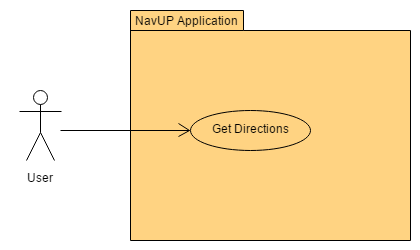
\includegraphics[height = 200px]{GetDesiredLocation.png}
				\end{figure}
			\end{enumerate}

		\begin{table}[htb]
			\centering
			\caption{UC1 -  Navigate user to their desired location}
			\label{my-label}
			\begin{tabular}{|l|l|}
				\hline
				\textbf{Actor: User} &
				\textbf{System: NavUP}
				 \\ \hline  & 0. The NavUP system displays the main window
				\\ \hline
				\begin{tabular}[c]{@{}l@{}}1. The user clicks on the navigation \\ button in the main menu\end{tabular}       &
				\begin{tabular}[c]{@{}l@{}}2. The system displays the navigation page to \\ the user\end{tabular}
				 \\ \hline
				\begin{tabular}[c]{@{}l@{}}3. The user clicks on the Get Directions button\\ on the Navigation page\end{tabular} & 
				\begin{tabular}[c]{@{}l@{}}4. The system prompts the user for their \\ required destination\end{tabular}
				\\ \hline
				5. User enters desired destination & 
				\begin{tabular}[c]{@{}l@{}}6. The system calculates and displays the route\\ and directions to the destination\end{tabular}
				\\ \hline
			\end{tabular}
		\end{table}
				%%%%%%%%%%%%%%%%%%%%%%======================   UC2    ================%%%%%%%%%%%%%%%%
		\newpage
		\subsubsection{Use Case for REQ1: Obtain Current Location}
			\begin{enumerate}
			\renewcommand{\labelenumi}{{\textbf{\arabic{enumi}.}}}
			\item Use Case ID: UC2
			\item Precondition: User is running the NavUP application and requires their location
			\item Postcondition: Client device recieves and displays the user's current location data.
			\item Actor-System interaction model:
				\graphicspath{ {./Diagrams/User/} }
				\begin{figure}[h]
				\caption{Use Case Diagram -  UC2  Obtain Current Location}
				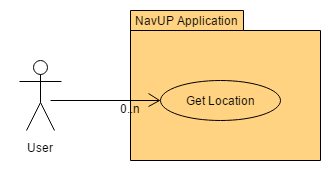
\includegraphics[height = 200px]{ObtainCurrentLocation.png}
				\end{figure}
			\end{enumerate}

		\begin{table}[htb]
			\centering
			\caption{UC2 -  Obtain Current Location}
			\label{my-label}
			\begin{tabular}{|l|l|}
				\hline
				\textbf{Actor: User} &
				\textbf{System: NavUP}
				 \\ \hline  & 0. The NavUP system displays the main window
				\\ \hline
				\begin{tabular}[c]{@{}l@{}}1. The user clicks on the navigation \\ button in the main menu\end{tabular}       &
				\begin{tabular}[c]{@{}l@{}}2. The system displays the navigation page to \\ the user\end{tabular}
				 \\ \hline
				\begin{tabular}[c]{@{}l@{}}3. The user clicks on the Get Location button\\ on the Navigation page\end{tabular} & 
				\begin{tabular}[c]{@{}l@{}}4. The system displays the user's location
				\end{tabular}
				\\ \hline
			\end{tabular}
		\end{table}
		
		
		%%%%%%%%%%%%%%%%%%%%%%======================   UC3    ================%%%%%%%%%%%%%%%%
		\newpage
		\subsubsection{Use Case for REQ1: Search for Location}
			\begin{enumerate}
			\renewcommand{\labelenumi}{{\textbf{\arabic{enumi}.}}}
			\item Use Case ID: UC3
			\item Precondition: User is running the NavUP application and searches for a given location.
			\item Postcondition: Information regarding  the searched location os provided.
			\item Actor-System interaction model:
				\graphicspath{ {./Diagrams/User/} }
				\begin{figure}[h]
				\caption{Use Case Diagram -  UC3  Search for location}
				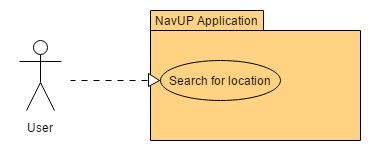
\includegraphics[height = 200px]{SearchForLocation.png}
				\end{figure}
			\end{enumerate}

		\begin{table}[htb]
			\centering
			\caption{UC3 -  Search for location}
			\label{my-label}
			\begin{tabular}{|l|l|}
				\hline
				\textbf{Actor: User} &
				\textbf{System: NavUP}
				 \\ \hline  & 0. The NavUP system displays the main window
				\\ \hline
				\begin{tabular}[c]{@{}l@{}}1. The user clicks on the navigation \\ button in the main menu\end{tabular}       &
				\begin{tabular}[c]{@{}l@{}}2. The system displays the navigation page to \\ the user\end{tabular}
				 \\ \hline
				\begin{tabular}[c]{@{}l@{}}3.  The user clicks on the Search for Location\\ button on the Navigation page\end{tabular} & 
				\begin{tabular}[c]{@{}l@{}}4. The system prompts the user for the \\ location they wish to search\end{tabular}
				\\ \hline
				5. User enters desired location & 
				\begin{tabular}[c]{@{}l@{}}6. The system provides information regarding \\ the searched location\end{tabular}
				\\ \hline
			\end{tabular}
		\end{table}

	\subsection{Entity Relationship Diagrams}

\newpage
%%%%%%%%%%%%%%%%%%%%%%%%%============= Specific Requirements ================%%%%%%%%%%%%%%%%%%%%%%%%%
\section{Specific Requirements}

	\subsection{External Interface Requirements}
		\subsubsection{User Interfaces}
		        The mobile application will interface with the supported input and output features of the host's operating system. Inputs include text that the user will enter for login or searching a venue. Outputs include the type of fonts to display text or graphics to show images or draw the map.

		\subsubsection{Hardware Interfaces}
			Since neither the mobile application nor the web portal have any designated hardware, it does not have any direct hardware interfaces. The WiFi software in the mobile phone manages the built-in WiFi and the hardware connection to the database server is managed by the underlying operating system on the mobile phone and the web server.

		\subsubsection{Software Interfaces}
			The mobile application communicates with the WiFi software in order to get signal strength information from multiple WiFi access points to determine (using triangulation) where the user is located. The communication software between the database and mobile application consists of operation concerning creating, reading, removing and modifying the data.

		\subsubsection{Communication Interfaces}
			The communication between the different parts of the system are important since they depend on each other. However, in what way the communication is achieved is not important for the system and is therefore handled by the underlying operating systems for both the mobile application and the back-end of the system.
	
		
	\subsection{Performance Requirements}
		\subsubsection{Performance}
			\begin{itemize}
			\item Offline activities should have a response time of +/- 2 seconds (instantaneous) when responding to an activity, while online activities such as calculating routes should have a response time of +/- 2-4 seconds so that the users have an uninterrupted experience.
			\item It should also allow the integration of a variety of services.\\
			\end{itemize}
			\subsubsection{Reliability} 
			\begin{itemize}
			\item It should be able to handle +/- 50 000 users concurrently (simultaneously) when implemented into a suitable production environment. 
			\item The application should be reliable, in that it will provide the fastest route every time without fail and complete all other computations successfully. 
			\item All activities should be completed with a 0.1 error allowance.
			\item The application should provide accurate locations in a constantly changing environment.\\
			\end{itemize}
			\subsubsection{Security}
			\begin{itemize}
			\item Data transmission should be securely transmitted without unauthorized access, or loss of information.\\
			\end{itemize}

	
	
	\subsection{Design Constraints}
		\begin{itemize}
				\item Security  - The users personal information and current location should not be accessible to the public.
				\item Accuracy - The users location should be found whether the user is indoors or not. The location of the user should also be found in terms of which floor they are on in the building.
				\item Performance - The system should be able to handle a large amount of users making use of the software at the same time, the system should also use resources on the client device efficiently.
				\item Reliability - The application should still operate when one or more data access points are no longer available.
				\item Accessibility - The application should be easily accessible to everyone that requires it.
				\item Usability - The applications interface should be easy to use and understand.
				\item Size - The application should not require too much memory in order to operate.
				\item Users - The nature of some users enforces constraints such as conforming to the WCAG for accessibility issues.
				\item Sensors - sensors attached to objects should be bluetooth enabled.
				\item Platform - the system should be accessible on  Android  devices.
				\item Modularity - The system should be modular, thus allowing for high cohesion with low coupling and reducing the dependencies within the system.
				\item Aesthetics - The system's interfaces should be aesthetically pleasing and follow the UP branding guidelines.
				\item Fault tolerance - if unavoidable malfunctions occurr,the design should be constrainted such that the system can recover without loss of data or damage.
				
			\end{itemize}
	
	\subsection{Software System Attributes}

		\subsubsection{Reliability}

			\begin{itemize}
				\item Any information that is stored on the database must remain correct when being transferred to the user interface.
				\item The services offered by the system should be available to users except for when the system is undergoing maintenance.
				\item The system should reply to user requests in the shortest time interval possible.
				\item The system must be fault tolerant, it needs to maintain a certain level of performance and offer other services that are not affected by this fault to the users.
				\item In the event of a fault the system must be able to recover within the shortest time period possible and recover any data that may have been lost.
				\item The system should be able to respond appropriately if it receives bad input data from the user.
			\end{itemize}

		\subsubsection{Scalability}
			\begin{itemize}
				\item The system must be able to cater for increases in the work load, for example large number of users or activities at any given time, without impacting the performance of the system.
				\item If the system does not cater for increases in workload it should at least provide the ability to be readily enlarged.
			\end{itemize}
		
		\subsubsection{Maintainability}
			\begin{itemize}
				\item The system must be designed in a modular fashion that provides high cohesion and loose coupling, this will allow parts of the system to be easily maintained without affecting the rest of the system.
				\item Maintenance should be able to be carried out by different maintenance teams, therefore the system must be easy to learn and understand.
			\end{itemize}

		\subsubsection{Integrability}
		
			\begin{itemize}
				\item] Since we are following a modular design, components of the system that are separately developed should work correctly together.
				\item Follow coding standards specified by the client to allow for easy integration and employ continuous integration in our design process.
			\end{itemize}
		
		\subsubsection{Usability}
		
			\begin{itemize}
				\item The system must be easy to learn.
				\item System must cater for user mistakes, by providing the user with the undo or roll back options.
				\item The user interface must be easy to use and must be intuitive.
				\item The system should display options in a logical manner.
				\item Incorporate widgets and icons that the target users may be familiar with.
				\item The user manual should have a detailed description of the system.
				\item A help option must be provided to the users.
			\end{itemize}
		
		\subsubsection{Interoperability}
			\begin{itemize}
				\item The system must be able to communicate with the University of Pretoria WiFi system, because the WiFi  access points will be used for the navigation.
			\end{itemize}

\end{document}
